\documentclass[]{article}
\usepackage{graphicx}
\usepackage[margin=1in]{geometry}

%opening
\title{EYIC IDEA PROPOSAL
	\linebreak 
	e-Yantra Ideas Competition 2019-20}
\date{}
\begin{document}
\maketitle{}
\section{Project Name:}
\subparagraph{SMART BUS MANAGEMENT}

\section{Introduction/Motivation:}
\subparagraph{Daily some inconvenience is confronted by users of various institutions due to Improper distribution of the control over the passenger carrier automobiles of their transport system. The Smart bus management system helps in efficient use of bus capacity, delivering passenger convenience with location and time management. It also contributes in conserving the environment by efficient fuel consumption.}


\section{Market Research / Literature Survey:}

\subsection{Customer Need Identification:}
\subparagraph{We have surveyed and analysed the probable market - institutions with high congestion bus facility. Thus, the data gathered so far reflects the need of creating a system towards improving fuel efficiency, crowd management, revenue collection etc.
}
\begin{figure}[h]
	\centering
	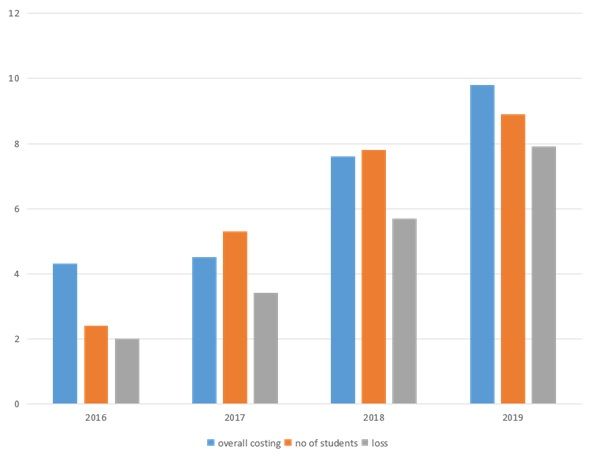
\includegraphics[width=0.5\linewidth,height=0.5\linewidth]{chart}
	\caption{fig:Bus Fee (Paid Vs Unpaid) Stats}
	\label{fig:Bus Fee (Paid Vs Unpaid) Stats}
\end{figure}


\subsection{Market Identification and Justification:}
\subparagraph{Our target consumer area is institutions with bus facilities, typically it can be personalized according to need fulfilment. The data says that an average institution faces major losses due high cost fuel wastage as well as insufficient revenue collection. The defaulters on other hand enjoy the advantages of these loop holes.
}

\subsection{Understanding of your customer and user:}
\subparagraph{As a project developer as well as consumer somehow, we see an enormous scope of this due project named as smart bus management. Since we are also a part on ongoing buggy system, we can see the market potential of project implementation.}

\section{Hardware requirements:}
\begin{itemize}
	\item Power Supply (adapters , SMPS etc.)
	\item PIC16F877A (dip package)
	\item Keypad (3X3)
	\item LCD oled ( 16X2)
	\item Lithium ion battery
	\item WiFi module (router)
	\item Buzzer
	\item RS 232 communication
	\item B-Type USB
	\item PCB with all sub portions
	\item Crystal oscillator
	\item Memory IC 
	\item CMOS cell	
\end{itemize}

\section{Software requirements:}
\begin{itemize}
\item MPLAB X
\item XC8 compiler
\item PIC boot-loader
\item Data Acquisition Toolbox 
\item Net-beans 8.2
\item JAVA 8
\item JSP
\item tomcat 7
\item HTML
\item PHP
\item Java Script
\item Heroku cloud
\item CSS - cascade style sheets
\item RDBMS - Relational Database Management System	
\end{itemize}

\section{Implementation:}
\subparagraph{A web-app based H/W is designed for tracking a transport vehicle and time-location calculations along its route. Tracking System involves the installation of an electronic device in a vehicle, with the web-app enabling all, the Administrator/User to track the bus location and estimate the arrival and departure time. By the application, the management or any authorized individual can check the validity and eligibility of the passenger entering the vehicle. There are two applications server and client. The System shows where the vehicle is on a map and provides passengers and management staff, the updated information at different time interval. It is a real-time system. PIC16F108 micro-controller is used to programming for interfacing the S/W and H/W module. It is connected to the cloud and hardware through the application. This application can be easily extended for the central GPS to keep track of all the vehicles. Different queries and efficient route management can be easily done through the central server system.}

\subparagraph{Our projects made technically innovative with an effective combination of hardware and software, providing the authority, a flexible source to access the management of their transport system with ease. Passengers are allowed to pre-book their seats on a selected route giving the exact data about number of students to the authority, which makes the product unique within itself. A web-app based H/W is designed for tracking a transport vehicle and time calculations along its route. Tracking System involves the installation of an electronic device in a vehicle, with a app enabling all, the Administrator/User to track the bus location. By the application, the management or any individual can check the validity and eligibility of the passenger.}

\begin{figure}[h]
	\centering
	
\includegraphics{user}
	\caption{User Side Web-App Structure}

\end{figure}
\begin{figure}[h]
	\centering
	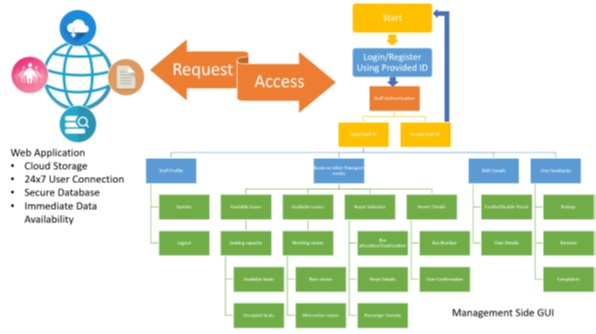
\includegraphics{management}
	\caption{Management Side Web-App Structure}

\end{figure}

\section{Feasibility:}
\subparagraph{We are developing a web application and a cos- effective hardware which is easily accessible by any user and staff member in any web browser that now a days everyone has access to, only they need is some basic and primary knowledge for accessing the web. The increasing number of individuals in institutions/organizations leads in mismanagement of the facilities distribution and resource utilization. To overcome this mismanagement effectively we swam in the digital ocean and are working on the digital transport management system. This will provide effective management of the transport provided by the institution/organization, as our project is about smartly handling the transport management related problems. The main motive of innovation in this project is for providing the most efficient distribution of facilities to those users who are eligible as they are paying for it and an effective utilization of the resources provided. These facilities are in the form of service, comfort, Eco-friendly resource consumption, beneficial for managing department and financial benefits.}

\section{References:}
\begin{itemize}
	\item Microchip : www.microchio.com
	\item http://www.microchio.com>PIC16F877A
	\item University Suggestion Box
	\item Faculty Guiding
	\item Survey ( Market Research)
\end{itemize}

\end{document}
